\cotefile{147}

\scanpage{24}
\mspage{11}
c'est une fonction localement constante sur $\mathcal S$.

Fixons nous un type numérique $(g,\nu)$\inserted{\uline{anabélien} $(2g+\nu\geq3)$}, et considérons, pour $\mathcal S$ variable, le groupoïde fibré
\[
(24)\qquad\mathcal S\longmapsto\widehat{M}_{g,\nu}(\mathcal S)=\begin{gathered}\text{MD-courbes}\\\text{\unsure{relatives|relives} sur }\mathcal S,\text{ de}\\\text{type numérique}\\\text{égal \unsure{à|:} }(g,\nu)\end{gathered}
\]
On a alors le vraiment mirifique théorème suivant :

\margin{On \unsure{suppose|supp\textsuperscript{se}} $2g+\nu\geq3$ (cas anabélien)}
\uline{Théorème} de \uline{Mumford-Deligne} : Le

\figure{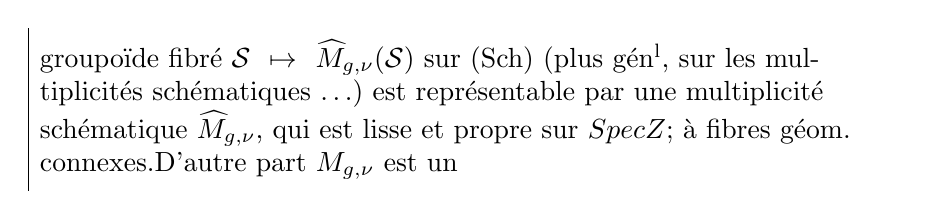
\begin{tikzpicture}
\node[anchor=north west,text width=0.9\linewidth,align=left,inner sep=4pt] (T) at (0,0) {
groupoïde fibré $\mathcal S\mapsto\widehat{M}_{g,\nu}(\mathcal S)$ sur $(\mathrm{Sch})$ (plus gén\textsuperscript{l}, sur les multiplicités schématiques $\ldots$) est représentable par une multiplicité schématique $\widehat{M}_{g,\nu}$, qui est \uline{lisse} et \uline{propre} sur $\operatorname{Spec}\mathbb Z$; \deleted{à fibres géom. connexes.}\inserted{D'autre part $M_{g,\nu}$ est un}
};
\draw[line width=0.5pt] (T.north west)--(T.south west);
\end{tikzpicture}}
\mspage{23}

\scanpage{26}
\mspage{12}
MD-graphe trivial, ayant un seul sommet de genre $g$, de poids marqué $\nu$, et pas d'arêtes, redonne l'immersion ouverte canonique
\[
(26)\qquadM_{g,\nu}\hookrightarrow\widehat{M}_{g,\nu}.
\]
Identifiant les $M_{[G]}$ à des sous-multiplicités de $\widehat{M}_{g,\nu}$, on voit que les $M_{[G]}$ (pour tous les types de \unsure{\deleted{\unsure{MD}}|M\deleted{\unsure{D}}}-graphes possibles, de type numérique $(g,\nu)$) forment une \uline{partition} de $\widehat{M}_{g,\nu}$ en un nb fini de sous-multiplicités.

\uline{Remarque} Considérons l'adhérence d'un $M_{[G]}$ dans $\widehat{M}_{g,\nu}$, on trouve que c'est une réunion finie de\deleted{\unsure{s}} $M_{[G']}$. On dit que $[G']$ est spécialisation de $[G]$ si $M_{G'}\subset\overline{M_G}$ dans $\widehat{M}_{g,\nu}$.
\mspage{25}

\scanpage{29}
avec un poids marqué \deleted{$\unsure{\nu}$}, \unsure{(}et bien sûr, un genre donné). Du pt de vue structure de graphe associé au type numérique $(g,\nu)$, c'est le plus simple de tous ! On étudiera les plus complexes tantôt, qui correspondent au cas d'une dimension modulaire nulle, \unsure{ie|\deleted{\unsure{ou}}et} d'une codimension modulaire maximale, égale à $3(g-1)+\nu$.

Il est tentant d'introduire le compactifié
\[
\widehat{\mathcal M}_G\overset{\mathrm{déf}}{=}\prod_{\alpha\in S}\widehat{\mathcal M}_{g_\alpha,\widehat I_\alpha}
\]
où les $\widehat{\mathcal M}_{g_\alpha,\widehat I_\alpha}$ sont les compactifiés de MD des $\mathcal M_{g_\alpha,\widehat I_\alpha}\simeq\mathcal M_{g_\alpha,\widehat\nu_\alpha}$. \deleted{\unsure{Ils|Il}}\inserted{Pour $\alpha$ fixé, $\widehat{\mathcal M}_{g_\alpha,\widehat I_\alpha}$} représente\deleted{\unsure{nt}} le groupoïde fibré
\[
(30)\qquad\begin{aligned}
\mathcal S\longmapsto&\ \text{courbes de MD relatives }\inserted{Y_\alpha}\text{ sur }\mathcal S,\\
&\text{de type }g_\alpha,\widehat I_\alpha\quad\text{i.e. de genre}\\
&g_\alpha,\text{ munies d'un mono}\\
&(\widehat I_\alpha)_{\mathcal S}\hookrightarrow Y_\alpha^{\text{lisse}}
\end{aligned}
\]
de sorte que $\widehat{\mathcal M}_G$ représente le groupoïde fibré
\mspage{28}

\scanpage{30}
\mspage{14}
\[
(31)\qquad\begin{aligned}
\mathcal S\longmapsto&\ \text{groupoïde des }\inserted{\text{systèmes }(Y_\alpha)_{\alpha\in S}\text{ de }}\text{courbes de MD}\\
&\inserted{Y_\alpha\text{ de genre }g_\alpha,}\ \text{\deleted{\unsure{à}} sur }\mathcal S,\text{ munies de mono.}\\
&\widehat I_{\alpha\mathcal S}\hookrightarrow Y_\alpha^{\text{lisse}}.
\end{aligned}
\]
Posant alors
\[
\underset{\text{\deleted{On aura}}}{(32)}\qquad\left\{\begin{aligned}
\widehat I&=\coprod\widehat I_\alpha\simeq I\amalg\widetilde A\\
Y&=\coprod_{\alpha\in S}Y_\alpha
\end{aligned}\right.
\]
on aura un mono
\[
(33)\qquad\widehat I_{\mathcal S}\hookrightarrow Y^{\text{lisse}}
\]
qui permet, d'une part de construire un
\[
(34)\qquad\overset{\deleted{\unsure{\wedge}}}{\mathcal X}=Y/\unsure{(\sigma)_{\deleted{\unsure{I}}\widetilde A_{\mathcal S}}|(\sigma_{\deleted{\unsure{I}}\widetilde A_{\mathcal S}})},
\]
qui sera manifestement une courbe \deleted{\unsure{standart}}\inserted{MD} sur $\mathcal S$, et d'autre part de définir
\[
(35)\qquad\overset{\deleted{\unsure{\wedge}}}{I}_{\mathcal S}\hookrightarrow\overset{\deleted{\unsure{\wedge}}}{\mathcal X}^{\text{lisse}}
\]
de sorte que $(\mathcal X,\overset{\deleted{\unsure{\wedge}}}{I}_{\mathcal S})$ devient une courbe \deleted{\unsure{standart} \unsure{sur} $\mathcal S$} MD sur $\mathcal S$, ``épinglée'' par l'ens fini $I$. On a donc un morphisme canonique de multiplicités
\[
(36)\qquad\widehat{\mathcal M}_G\longrightarrow\widehat{\mathcal M}_{g,I}
\]
\margin{\uline{NB} Ce morphisme est une imm. locale, mais pas une immersion [il ne correspond pas à un morphisme pl. fid. des gr. à priori définis]}
compatible d'ailleurs avec l'action de $\Gamma=\operatorname{Aut}G$ sur $\widehat{\mathcal M}_G$, et son action sur $\widehat{\mathcal M}_{g,I}$ via $\Gamma\to\mathfrak S_I$.
\mspage{29}

\scanpage{31}
On en déduit donc un morphisme can. de multiplicités schématiques
\[
(37)\qquad
\diagram{\begin{tikzcd}[column sep=large,row sep=small]
\widehat{\mathcal M}_{[G]}\arrow[r,hook]&\widehat{\mathcal M}_{g,\nu}\\
(\widehat{\mathcal M}_G,\Gamma)\arrow[u,phantom,"{\wr\,|\ \mathrm{déf}}" description] & (\widehat{\mathcal M}_{g,I},\mathfrak S_I)\arrow[u,phantom,"{\wr\,|}" description]
\end{tikzcd}}
,
\]
qui est encore une \uline{immersion}, fermée cette fois-ci, de multiplicités schématiques propres et lisses sur $\mathbb Z$. Ainsi se trouve explicité l'adhérence de $\mathcal M_{[G]}$ dans $\widehat{\mathcal M}_{g,\nu}$, \deleted{comme} sous-multiplicité propre et lisse sur $\operatorname{Spec}\mathbb Z$ -- qui \unsure{paraît} \inserted{a priori} curieux ! En $=$ temps, cette construction permet de décrire de façon pratiquement triviale les types $[G']$ qui sont spécialisation de $[G]$, puisque ce sont ceux qui proviennent de $\widehat{\mathcal M}_G$. Nous allons \deleted{\unsure{y}} revenir là dessus maintenant.
\mspage{30}

\scanpage{32}
\mspage{15}
5. \uline{Spécialisation \deleted{et générisation} de MD-graphes.}

Soit
\figure{\begin{tikzpicture}[baseline=(f.base)]
\node[inner sep=7pt] (f) {$G=(S,\widetilde A,\sigma_{\widetilde A},\overset{\deleted{\unsure{\sigma_{\widetilde A}|\widetilde A}}}{I},\ \underset{\substack{\Vert\\\widetilde A\amalg I}}{\widehat I}\to S\xrightarrow[g]{}\deleted{\unsure{g}}\mathbb N)$};
\node[anchor=east] at ([xshift=.05cm,yshift=-.12cm]f.west) {$(38)$};
\draw ([xshift=-.5cm]f.south west)--(f.south west)--(f.north west)--(f.north east)--(f.south east)--([xshift=.1cm]f.south east);
\end{tikzpicture}}
un MD-graphe, de type numérique $(g,\nu)$. Nous allons construire ses \deleted{$\unsure{g|G}$} spécialisations, \deleted{comme} les \inserted{MD-}graphes associés aux diverses ``strates'' de
\[
\deleted{\unsure{\widehat{\mathcal M}_G}}\qquad\widehat{\mathcal M}_G=\prod_{\alpha\in S}\widehat{\mathcal M}_{g_\alpha,\widehat I_\alpha}.
\]
Une telle strate est obtenue en choisissant, pour $\forall\ \alpha$, une strate de $\widehat{\mathcal M}_{g_\alpha,\widehat I_\alpha}$, c'est à dire une classe d'isomorphie de MD-graphes
\deleted{$G_\alpha=(S(\alpha),\widetilde A(\alpha),\sigma_{\widetilde A(\alpha)},\ I(\alpha)=\widehat I_\alpha\to S(\alpha)\to\mathbb N)$ de type numérique}
de type \deleted{$(g_\alpha,\widehat\nu_\alpha)$} numérique $(g_\alpha,\widehat I_\alpha)$
\[
(39)\quad\deleted{\unsure{(g_\alpha,\widehat\nu_\alpha)}}:\quad
\begin{aligned}
G(\alpha)=(S(\alpha),\widetilde A(\alpha),\sigma_{\widetilde A(\alpha)},\ &I(\alpha)=\widehat I_\alpha,\\
&\deleted{\unsure{\widehat I(\alpha)\amalg\widetilde A(\alpha)\to S(\alpha)}\xrightarrow{\unsure{\sigma_\alpha|g_\alpha}}\mathbb N}\\
&\inserted{\widehat I(\alpha)\overset{\mathrm{déf}}{=}\unsure{\widehat A(\alpha)|\widetilde A(\alpha)}\amalg I(\alpha)\to S(\alpha)\xrightarrow{\unsure{\sigma_\alpha|g_\alpha}}\mathbb N})
\end{aligned}
\]
(\uline{NB} bien entendu, le cas où $G(\alpha)$ est le MD-graphe trivial de type $(g_\alpha,\widehat\nu_\alpha)$ n'est pas exclu).

Par ``classes d'isomorphie'', il faut entendre ici : pour des isomorphismes induisant l'identité sur $I(\alpha)=\widehat I_\alpha$. Au lieu de travailler avec de telles classes d'isomorphie, nous allons pour commencer travailler
\mspage{31}

\scanpage{33}
avec ces $G(\alpha)$ eux-mêmes.

Le \inserted{MD-}graphe \inserted{$G'$} spécialisé de $G$ associé aux $G(\alpha)$ s'obtient ainsi :
\[
(40)\quad\left\{\begin{aligned}
S'&=\coprod_{\alpha\in S}S(\alpha)\\
\widetilde A'&=\widetilde A\amalg\coprod_{\alpha\in S}\widetilde A(\alpha)\\
\sigma_{\widetilde A'}&\quad\text{induit par }\sigma_{\widetilde A}\text{ et par les }\sigma_{\widetilde A(\alpha)}\\
&\deleted{\unsure{\widetilde A'}}\\
I'&=I\quad\text{donc }\begin{aligned}[t]
&\inserted{\widehat I'\overset{\mathrm{déf}}{=}}\widetilde A'\amalg I'\simeq\underbrace{(\widetilde A\amalg I)}_{\widehat I\simeq\coprod_{\alpha\in S}\widehat I_\alpha=\coprod_{\alpha\in S}I(\alpha)}\amalg\coprod_{\alpha\in S}\widetilde A(\alpha)\\
&\deleted{\unsure{=}}\simeq\coprod_{\alpha\in S}\unsure{\underbrace{\widehat I_\alpha\amalg\widetilde A(\alpha)}_{I(\alpha)}}
\end{aligned}\\
&\deleted{\unsure{\widehat I'\amalg\widetilde A'|I'\amalg\widetilde A'}}.\\
\widehat I'&\to S'\quad\text{induit par les }\widehat I(\alpha)\to S(\alpha)\\
S'&\xrightarrow{g'}\mathbb N\quad\text{induit par les }S(\alpha)\xrightarrow{\deleted{\unsure{g_\alpha}}}\mathbb N
\end{aligned}\right.
\]
Donc ``la ''recette \inserted{pratique''} est la suivante :

\deleted{\unsure{y}} On remplace chaque sommet \inserted{$\alpha\in S$} de $G$ par un MD-graphe $G(\alpha)$, de type numérique $(g_\alpha,\widehat\nu_\alpha)$, où $\widehat\nu_\alpha=\nu_\alpha+\widetilde\mu_\alpha$ ($\nu_\alpha=\operatorname{card}I_\alpha$, poids marqué de $\alpha$, $\unsure{\widehat\mu_\alpha|\widetilde\mu_\alpha}=\text{ordre de }\alpha=\text{nb }\text{d'arcs}\text{ de }G\text{ sortant de }\alpha$), plus précisément, un MD-graphe de type $(g_\alpha,\widehat I_\alpha)$, où $\widehat I_\alpha=I_\alpha\amalg\widetilde A_\alpha$.
\mspage{32}

\scanpage{34}
\mspage{16}
Cela signifie qu'on se donne, pour $\alpha$ fixé,

1°) un graphe \inserted{connexe} $(S(\alpha),\widetilde A(\alpha),\deleted{\unsure{\widetilde A(\alpha)}}\sigma_{\widetilde A(\alpha)},\widetilde A(\alpha)\to S(\alpha))$

2°) on \deleted{\unsure{fix|se}} donne une application ``genre''
\[
S(\alpha)\xrightarrow{\gamma_\alpha}\mathbb N
\]

3°) on donne une application $I_\alpha\to S(\alpha)$, i.e. on ``répartit'' les \deleted{\unsure{divers}} ``pts marqués'' au dessus de $\alpha$ \inserted{(i.e. les éléments de $I_\alpha$)} entre les sommets $\beta\in S(\alpha)$ de $G(\alpha)$

4°) on donne une application $\widetilde A_\alpha\to S(\alpha)$, i.e. pour tt \deleted{flèche}\inserted{arc} du graphe $G$, d'origine $\alpha$, on \deleted{\unsure{se donne}} ``choisit une \inserted{nouvelle} origine'' parmi les sommets $\beta\in S(\alpha)$ du graphe $G(\alpha)$

5°) Les données 1°) : 4°) définissent une maquette, \inserted{0-connexe, $G(\alpha)$} et on prend soin que celle-ci soit un MD-graphe, \deleted{\unsure{ce}} ce qui signifie ici pour pour tt $\beta\in S(\alpha)$ ``de genre 0'' i.e. tel que $\gamma_\alpha(\beta)=0$, on ait $\operatorname{card}I_{\alpha,\beta}+\operatorname{card}\widetilde A_{\alpha,\beta}\geq 3$.

Ceci étant, on trouve un nouveau \inserted{MD-}graphe\inserted{$G'$}, \inserted{qui sera} spécialisé du \inserted{MD-}graphe $G$.

Je voudrais préciser de façon simplifiée la relation entre les MD-graphes $G$ et $G'$, et j'introduis à cet effet une digression sur
\mspage{33}

\scanpage{35}
une extension de la notion de \uline{morphismes de graphes}.

\deleted{\unsure{6}}\qquad\deleted{Soit}

6. \uline{Morphismes de générisation de graphes \deleted{\unsure{ordinaires|quelconques}}\inserted{et de maquettes}}

Soit $G=(S,\widetilde A,\sigma_{\widetilde A},o_{\widetilde A}:\widetilde A\unsure{\to|{-}}S)$ un graphe ordinaire. On lui associe de façon bien connue un \uline{groupoïde fondamental} \inserted{$\Pi_1(G)$}, dont l'ens des objets est $S$, et l'ens des \deleted{\unsure{chemins de}}\inserted{morphismes} de $s$ à $s'$ est l'ens des ``chemins simples'' de $s$ à $s'$, qui correspondent aux classes d'homotopie de chemins de $s$ à $s'$ dans la réalisation topologique du graphe $G$. Le groupoïde $\Pi_1(G)$ dépend fonctoriellement (au sens le plus strict !) du graphe $G$.

D'ailleurs, un morphisme de graphes
\[
(41)\qquad f:G'\longrightarrow G^{\deleted{\unsure{'|''}}}
\]
\mspage{34}

\scanpage{37}
comme étant les morphismes de groupoïdes $\Pi_1(G')-\Pi_1(G^{\deleted{\unsure{'}}})$ qui transforment tout arc de $G'$ en une flèche de $\Pi_1(G)$ qui est, \uline{soit} un arc de $G^{\deleted{\unsure{'}}}$, soit une flèche identique. En d'autres termes, appelant \uline{flèche élémentaire} de $\Pi_1(G')$ tt flèche qui est, soit identique, soit un arc de $G'$ (ensemble \inserted{de flèches} stable par passage à la flèche opposée\ldots), les morphismes \deleted{de} \deleted{\unsure{générisation}}\inserted{\unsure{généralisés}} de $G'$ dans $G^{\deleted{\unsure{'}}}$ sont les morphismes de $\Pi_1(G')$ dans $\Pi_1(G)$ qui transforment fls élémentaires en fl. élémentaires. Cette description a l'avantage de rendre évident que cette notion est stable par composition.

Pratiquement, la donnée d'un morphisme \deleted{de} \deleted{\unsure{générisation}}\inserted{\unsure{généralisé}} \deleted{\unsure{de}} $G'\longrightarrow G^{\deleted{\unsure{'}}}$ est \unsure{défini|définie}
\mspage{36}

\scanpage{38}
\mspage{18}
par une application
\[
(44)\qquad S'\amalg\widetilde A'\longrightarrow S^{\deleted{\unsure{'}}}\amalg\widetilde A^{\deleted{\unsure{'}}}
\]
qui applique $S'$ dans $S^{\deleted{\unsure{'}}}$ (mais pas néc. $\widetilde A'$ dans $\widetilde A^{\deleted{\unsure{'}}}$), qui commute à $\sigma_{G'}$ et $\sigma_{G^{\deleted{\unsure{'}}}}$ (définis via $\sigma_{\widetilde A'}$ et $\sigma_{\widetilde A^{\deleted{\unsure{'}}}}$, avec l'identité sur $S'$ resp. $S^{\deleted{\unsure{'}}}$) et commute à l'application ``origine'' (qui sur $S'$ resp. $S^{\deleted{\unsure{'}}}$ est l'identité).

On peut aussi dire que c'est défini par la donnée
\[
(45)\quad\left\{\begin{aligned}
&\text{1°) d'une application}\qquad f_{\unsure{S|S^0}}:S'\longrightarrow S^{\deleted{\unsure{'}}}\\
&\text{2°) d'une partie }\deleted{\widetilde A}\widetilde B^{\prime\deleted{\unsure{'}}}\text{ de }\widetilde A',\text{ stable par }\sigma_{\widetilde A'}\\
&\text{3°) d'une application }\widetilde B'\to\widetilde A^{\deleted{\unsure{'}}}\text{ commutant à }\deleted{\unsure{\sigma}}\\
&\qquad\unsure{\text{à}}\ \sigma_{\widetilde A'}|\widetilde B'\text{ et à }\sigma_{\widetilde A^{\deleted{\unsure{'}}}},\text{ et aux applications}\\
&\qquad o_{\widetilde A'}|\widetilde B'\text{ et }o_{\widetilde A^{\deleted{\unsure{'}}}}.
\end{aligned}\right.
\]
\margin{et il faut supposer de plus que pour tt $\vec a\in\widetilde A'\setminus\widetilde B'$, l'origine et l'extrémité de $\vec a$ ont $\overline m$ image dans $S$ par $f_S$}

On peut dire enfin que c'est aussi la donnée d'un sous-graphe $G_{\widetilde B'}$ de \deleted{\unsure{$G$}}$G'$ ayant $=_{\mathrm s}$ sommets (cela défini juste \unsure{rev.|un} à donner une partie $\widetilde B'$ de $\widetilde A'$ stable par $\sigma_{\widetilde A'}$), et un morphisme de $G_{\widetilde B'}$ dans $G^{\deleted{\unsure{'}}}$. La composition des morphismes généralisés est alors définie et lue de façon
\mspage{37}

\scanpage{39}
évidente. Ainsi on trouve la catégorie \unsure{étendue} des graphes, dont les objets sont les graphes, les \deleted{\unsure{morphismes}}\inserted{flèches} les morphismes généralisés de graphes. On notera que les iso. dans cette nouvelle catégorie sont les iso au sens ordinaire.

Supposons maintenant que $G',G^{\deleted{\unsure{'|''}}}$ fassent partie de MD-graphes \inserted{$\underline G',\underline G^{\deleted{\unsure{'|''}}}$}, i.e. soient munis de plus de \deleted{$S\xrightarrow{g}\mathbb N$},
\[
(46)\quad\left\{\begin{aligned}
&S\overset{\underline g}{-}\mathbb N,\qquad S'\xrightarrow{\underline{g'}}\mathbb N\\
&I\longrightarrow S,\qquad I'\longrightarrow S'
\end{aligned}\right.
\]
On dit qu'on a un \uline{morphisme de générisation} de $\underline G'$ dans $\underline G^{\deleted{\unsure{'|''}}}$, si on se donne, en plus du morphisme \inserted{généralisé} $G'\to G^{\deleted{\unsure{'|''}}}$, une application bijective
\[
(47)\qquad I'\xrightarrow{\sim}I^{\deleted{\unsure{'|''}}},
\]
\deleted{\unsure{satisfai|satisfa}} et si les conditions suivantes sont satisfaites :
\mspage{38}

\scanpage{40}
\mspage{19}
a) $S'\longrightarrow S^{\deleted{\unsure{'}}}$ surjectif, $\widetilde B'\longrightarrow\widetilde A^{\deleted{\unsure{'}}}$ \uline{bijectif}

b) \diagram{\begin{tikzcd}
I'\arrow[r,"\sim"]\arrow[d]&I\arrow[d]\\
S'\arrow[r]&S
\end{tikzcd}} commutatif

\margin{donc \diagram{\begin{tikzcd}
\widetilde B'\amalg I'\arrow[r,"\sim"]\arrow[d]&\widetilde A\amalg I\arrow[d]\\
S'\arrow[r]&S
\end{tikzcd}} est comm.}

c) $\forall\alpha\in S$, le sous-graphe $G'(\alpha)$ de $G'$ [formé des \deleted{\unsure{$S$}} $s'\in S'$ au dessus de $\alpha$, et des \deleted{flèches} arcs $a'\in\widetilde A'$ qui sont dans $\inserted{\widetilde C'=}\widetilde A'\setminus\widetilde B'$ (i.e. au dessus de $\operatorname{id}_\alpha$) et dont l'origine (donc l'extrémité aussi) est dans $S'_\alpha$], muni de \deleted{\unsure{et par} $\unsure{\widetilde A_\alpha|\widetilde A}$ \unsure{ou|et} $\unsure{A}$} $I'_\alpha\inserted{\amalg\widetilde B'_\alpha}\longrightarrow S'_\alpha$ induit par $\inserted{\widetilde B'\amalg}I'\unsure{\to|{-}}S'$, et de $\gamma_\alpha:S'_\alpha\longrightarrow\mathbb N$ induit par $\unsure{g'|f'}:S'\unsure{\to|{-}}\mathbb N$, est un \uline{MD-graphe} \inserted{$\underline G'(\alpha)$} \deleted{\unsure{de type|de genre} $\unsure{g=g(\alpha)|(g_\alpha,\nu_\alpha)}$\unsure{, i.e.}}, i.e. il est \uline{connexe}, \deleted{[NB il \unsure{satisfait automatiquement}} \inserted{et [il satisfait tous}\deleted{\unsure{les}} \inserted{les} conditions de rigidité relatives aux sommets $\beta$ tels que, \deleted{\unsure{$\alpha$}} $g'_\beta\in\{0,1\}$, à savoir que

\margin{\uline{NB} $\widetilde B'_\alpha$ est l'ens des $\vec a'\in\widetilde B'_\alpha$ dont l'origine se trouve dans $S'_\alpha$, i.e. dans $G'(\alpha)$, donc $\widetilde B'_\alpha\xrightarrow{\sim}\widetilde A_\alpha$}

\figure{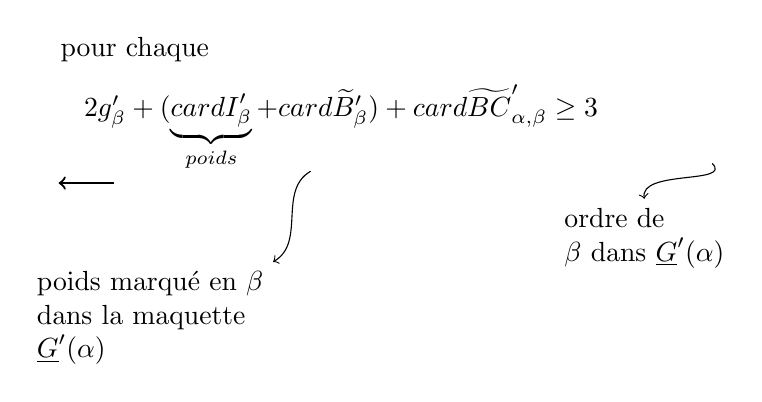
\begin{tikzpicture}[x=1cm,y=1cm]
\node[anchor=west] (eq) at (0,0) {$2g'_\beta+(\underbrace{\operatorname{card}I'_\beta}_{\deleted{\unsure{poids}}}\inserted{+\operatorname{card}\widetilde B'_\beta)}+\operatorname{card}\widetilde{\deleted{B}\inserted{C}}'_{\deleted{\unsure{\alpha}},\beta}\geq3$};
\node[anchor=north west,align=left] (mark) at (-0.6,-1.7) {poids marqué en $\beta$\\dans la maquette\\$\underline G'(\alpha)$};
\node[anchor=north west,align=left] (ord) at (6.1,-0.9) {ordre de\\$\beta$ dans $\underline G'(\alpha)$};
\draw[->,thick] (0.5,-0.7)--(-0.2,-0.7);
\draw[->] (3.0,-0.55) to[out=210,in=30] (mark.north east);
\draw[->] (8.1,-0.45) to[out=-45,in=100] (ord.north);
\node[anchor=west] at (-0.3,1.0) {\deleted{\unsure{pour chaque}}};
\end{tikzpicture}}

\margin{car la condition est \unsure{aut. assur.} \deleted{\unsure{a priori} $\unsure{2g'_\beta}$ \unsure{est}} \deleted{\unsure{puisqu'il est}} \unsure{équiv à} : \figure{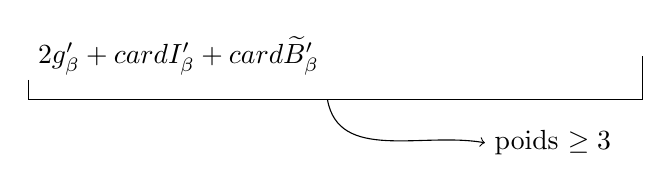
\begin{tikzpicture}[x=1cm,y=1cm]
\node[anchor=west] at (0,0) {$2g'_\beta+\operatorname{card}I'_\beta+\operatorname{card}\widetilde B'_\beta$};
\draw (0,-0.3)--(0,-0.55)--(7.8,-0.55)--(7.8,0);
\draw[->] (3.8,-0.55) to[out=-80,in=170] (5.8,-1.1);
\node[anchor=west] at (5.8,-1.1) {poids $\geq3$};
\end{tikzpicture}}}

\margin{\unsure{\deleted{$\operatorname{card}I_\beta$}}}

\deleted{\unsure{qui a priori} \unsure{$+\operatorname{car}$} $\left[2g'_\beta+\operatorname{card}I'_\beta\geq3\right]$ $2g'_\beta+\operatorname{card}I'_\beta+\operatorname{card}\widetilde A'_\beta\geq3)$ qui a priori est une condition plus faible (puisque $\underline G'$ est un MD-graphe)\ldots}

d) le genre du MD-graphe $\underline G(\alpha)$ est égal à $g_\alpha$, i.e. on a
\[
\sum_{\beta\in S'_\alpha}g'_\beta+h_1(G(\alpha))=g_\alpha.
\]
\mspage{39}

\scanpage{41}
\uline{NB} Pour qu'un morphisme généralisé de graphes $G'\deleted{\unsure{\text{et}}}\longrightarrow G$ corresponde à un morphisme de générisation (pour $I'\simeq I$ convenable), il f. et s. qu'il satisfasse aux conditions suivantes
\[
(48)\quad\left\{\begin{aligned}
&\text{1°) }S'-S\text{ surjectif},\quad\widetilde B'\longrightarrow\widetilde A\text{ bijectif, les}\\
&\qquad\inserted{\text{``graphes}}\text{ fibres'' }G'(\alpha)\quad(\alpha\in S)\text{ connexes. (Ces}\\
&\qquad\text{conditions ne dépendent pas des MD-}\\
&\qquad\text{structures sur }G',G\text{)}\\[1em]
&\text{2°) }\forall\alpha\in S,\text{ on a}\\
&\qquad\underbrace{\operatorname{card}I_\alpha}_{\nu_\alpha}=\sum_{\beta\in S'_\alpha}\underbrace{\operatorname{card}I'_\beta}_{\nu'_\beta}\\
&\qquad\text{(cette condition ne dépend que des}\\
&\qquad\text{``poids marqués'' sur }\unsure{\widehat S|S},S',\text{ et bien sûr}\\
&\qquad\text{de }S'-S\text{)}\\[1em]
&\text{3°)}\quad\forall\alpha\in S,\text{ on a}\\
&\qquad g_\alpha=\Big(\sum_{\beta\in S'_\alpha}g'_\beta\Big)+h_1(G'(\alpha))\\[1em]
&\deleted{\unsure{\text{4°)}}\quad\forall\unsure{\beta|\alpha'}\in S',\text{ on a (non seulement}}\\
&\deleted{\quad2g'_{\alpha'}+\operatorname{card}I'_{\alpha'}+\operatorname{card}\widetilde A'_{\beta'}\geq3,\text{ mais même)}}\\
&\deleted{\qquad\unsure{2|7}g'_{\alpha}+\operatorname{card}I'_{\alpha'}+\operatorname{card}\unsure{\widetilde C'|\widetilde B'}_{\alpha'}\geq3}
\end{aligned}\right.
\]
\mspage{40}

\scanpage{42}
\mspage{20}
Reprenons un morphisme généralisé de graphes ordinaires $f:G'_{\unsure{,|\bullet}}\to G^{\deleted{\unsure{'}}}$. On dit que $f$ est un \uline{morphisme de générisation} s'il satisfait la condition 1°) de (48). Notons que $G$ et $f$ sont définis alors à iso près par $G'$ et l'ens $\widetilde B'\subset\widetilde A'$ (stable par $\sigma_{\widetilde A'}$), ou ce qui revient au $\unsure{=|\overline m}$, par $G'$ et la \deleted{\unsure{ens}} partie $B'$ de $A'=\widetilde A'/\sigma_{\widetilde A'}$ ($B'$ est donc un ens. d'arêtes de $G'$). En effet, soit $G'_\bullet$ le sous-graphe de $G'$ défini par $S'$ et $A'\setminus B'\subset A'$ (ou $\widetilde A'\setminus\widetilde B'\subset\widetilde A'$) (i.e. \inserted{par $S'$ et} l'ens des \deleted{arêtes} arcs de $G'$ qui sont au dessus des identités de $\Pi_1(G)$). Alors il résulte de la condition $S'{-}S$ surjectif \inserted{et} les $G'(\alpha)$ connexes ($\Longleftrightarrow$ les $G'(\alpha)$ 0-connexes) que \deleted{les fibres} l'homomorphisme canonique
\[
\pi_0(G'_\bullet)\longrightarrow S
\]
est bijectif, d'où
\[
(49)\qquad S\simeq\pi_0(G'_\bullet),
\]
d'ailleurs on a
\[
(50)\qquad\widetilde A^{\deleted{\unsure{'}}}\simeq\widetilde B'\qquad\deleted{\unsure{\mathrm c}}\text{compatible avec }\sigma_{\widetilde B'}\text{ et }\sigma_{\widetilde A}
\]
\mspage{41}

\scanpage{43}
enfin $\widetilde A\xrightarrow{\sigma_G}S$ est donné par passage au quotient à partir de $\unsure{o_G|\sigma_G}|\widetilde B':\widetilde B'\to S'$, par commutativité dans

(51)\quad\diagram{\begin{tikzcd}
\widetilde B'\arrow[r,"o_{G'}|\widetilde B'"]\arrow[d,"\wr"']&S'=\text{sommets de }G'_\bullet\arrow[d]\\
\widetilde A\arrow[r]&S\simeq\pi_0(G'_\bullet)
\end{tikzcd}}

Ainsi $G$ est reconstruit à partir de $G'$, et $f$ de $\overline m$ bien sûr. On voit que $G$ apparaît comme un quotient de $G'$, et en fait c'est \unsure{plus|bien} une somme amalgamée dans la catégorie des graphes et des morphismes généralisés de graphes :

(52)\quad\diagram{\begin{tikzcd}[column sep=large,row sep=large]
G'_\bullet\arrow[r,hook,"\text{incl. can}"]\arrow[d,"\text{proj. can}"']\arrow[dr,phantom,"\text{cocart}"]&G'\arrow[d]\\
\begin{gathered}[t]S=\pi_0(\unsure{G'_\bullet|S'_\bullet})\\
\text{\unsure{(graphe|Graphe} }\deleted{\unsure{\text{ponctuel}}}\inserted{\text{discret}}\\
\text{défini par }S\overset{\mathrm{dfn}}{=}\pi_0(G'_\bullet)
\end{gathered}\arrow[r,Rightarrow]&G
\end{tikzcd}}

i.e. $G'\longrightarrow G$ est universel parmi les morphismes généralisés de \inserted{$G$ dans un} graphe $G'$, qui transforment les arcs de $\widetilde A'\setminus\widetilde B'$ en des identités. Posons donc
\mspage{42}

\scanpage{44}
\mspage{21}
\[
(53)\qquad\widetilde C'=\widetilde A'\setminus\widetilde B',\qquad C'=A'\setminus B'=\widetilde C'/\sigma_{\widetilde A'},
\]
on écrira
\[
(54)\qquad G=G'/\widetilde C'\quad\text{ou}\quad G=G'/C'
\]
et on dira que $G$ \uline{est déduit de} $G'$ en contractant les arêtes $a'\in C'$ (ou encore, les arcs $\vec a'\in\widetilde C'$) en des pts. Interprétant les morphismes généralisés de graphes, en termes des réalisations \deleted{géométriques}\inserted{topologiques} de ceux-ci, à l'aide d'applications continues qui contractent \unsure{juste|justement} certaines arêtes en des pts, on voit que cette terminologie correspond bien à une intuition topologique correcte. D'ailleurs la somme amalgamée (52) existe quel que soit le sous-graphe $G'_\bullet$ de $G'$ ayant $=_{\mathrm s}$ sommets que $G'$, i.e. quel que soit l'ens d'\deleted{\unsure{flèches}}\inserted{arêtes} $C'\subset A'$- de $G'_{\deleted{\unsure{\psi|\alpha}}\bullet}$. [Il s'ensuit que tout morphisme généralisé de graphes $G'\longrightarrow G$ se factorise de façon unique en un
\mspage{43}

\scanpage{45}
composé
\[
(55)\qquad G'\longrightarrow G_0\unsure{\longrightarrow|{-}}G,
\]
où $G'\unsure{\to|{-}}G_0$ est un morphisme de passage au quotient (par l'ens des arêtes de $\unsure{C'|G'}$ contractées par $f$, justement) et où $G_0\longrightarrow G$ est un morphisme \inserted{ordinaire} de graphes.

Supposons maintenant que $G'$ \inserted{soit fixé, et} \deleted{soit} provienne \inserted{$\overline m$} d'un MD-graphe $\underline G'$, grâce aux données supplémentaires
\[
\deleted{\unsure{(55)|(56)}}\qquad I'\longrightarrow S',\xrightarrow{\unsure{g'|\underline{g'}}}\mathbb N,
\]
où $I'$ est un ens. fini. Alors $G$ provient canoniquement d'un MD-graphe $\underline G$, en posant $I=I_{\underline G}=I'$, et en définissant $\unsure{I|I'}\unsure{\to|{-}}S$ comme le composé
\[
\underset{\substack{\Vert\,\mathrm{def}\\I}}{I'}\longrightarrow S'\longrightarrow S,
\]
et en définissant, pour $\forall\alpha\in S$
\[
(56)\qquad g_\alpha=\Big(\sum_{\alpha'\in\underset{\substack{\Vert\\\text{Sommets}\\\text{de }G'(\alpha)}}{S'_\alpha}}g'_{\alpha'}\Big)+h^1(G'(\alpha)).
\]
\mspage{44}

\scanpage{46}
\mspage{22}
Il faut cependant vérifier encore la condition MD sur la maquette $\underline G$ obtenue. Que $\underline G$ soit connexe résulte aussitôt de la connexité de $\underline G'$. Pour $\forall\alpha\in S$, il faut vérifier que
\[
2g_\alpha+\underbrace{\operatorname{card}I_\alpha+\operatorname{card}\widetilde A_\alpha}_{\widehat\nu_\alpha}\geq3
\]
\deleted{\unsure{or je dis qu'on aura mieux|ou je dis qu'on aura même}}

\deleted{ou}\inserted{i.e.} que $(g_\alpha,\widehat\nu_\alpha)$ est anabélien. Or
\[
\deleted{\operatorname{card}2g_\alpha+\operatorname{card}I_\alpha\geq3}
\]
\deleted{\unsure{je dis|je dit}}\inserted{on sait} que $(g_\alpha,\widehat\nu_\alpha)$ est le type numérique de la maquette $\underline G^{\deleted{\unsure{'}}}(\alpha)$, dont le graphe sous-jacent est la composante connexe de $G'_\bullet$ correspondant à $\alpha$, et l'ens. des ``pts marqués'' est $I'_\alpha\amalg\deleted{\unsure{\widetilde A}}\inserted{\widetilde B}'_\alpha$, \deleted{\unsure{et|à}} où $I'_\alpha=I'|S'_\alpha\simeq I_\alpha$, et $\widetilde B'_\alpha=\deleted{\unsure{\widetilde B|\widetilde A}}\inserted{\unsure{\widetilde A|\widetilde B}}'_\alpha\cap\widetilde B'$ est l'ens des flèches \unsure{de|$\in$} $\widetilde B'$ d'origine dans $S'_\alpha$, l'hom de projection
\[
I(\alpha)^{\deleted{\unsure{\ast|\alpha}}}\overset{\mathrm{def.}}{=}I'_\alpha\amalg\widetilde B'_\alpha\longrightarrow S'_\alpha
\]
étant induit par $I'\unsure{{-}|\to}S'$ et l'application origine. Donc, en vertu de la prop. du n° 3, on aura $(g_\alpha,\widehat\nu_\alpha)$ anabélien pourvu qu'on sache que $\underline G(\alpha)$ est un MD-graphe. Mais cette condition signifie que l'on a, pour $\forall\beta\in S'_{\deleted{\unsure{\beta|\alpha'}}\inserted{\alpha}}$
\mspage{45}

\scanpage{47}
\[
2g'_\beta+\underbrace{\bigl(\operatorname{card}I'_\beta\deleted{\unsure{(\alpha)}}+\operatorname{card}\widetilde B'_\beta\bigr)}_{\substack{\text{poids marqué}\\\text{de }\beta\text{ dans }\underline G(\alpha)}}+\underbrace{\operatorname{card}\widetilde C'_\beta}_{\substack{\text{ordre de}\\\beta\text{ dans }\underline G(\alpha)}}\geq3
\]
or cette expression s'écrit aussi, puisque
\[
\widetilde A'=\widetilde B'\amalg\widetilde C'
\]
\[
2g'_\beta+\underbrace{\operatorname{card}I'_\beta}_{\substack{\text{poids marqué}\\\text{de }\beta\text{ dans }\underline G'\deleted{\unsure{\alpha|\xi}}}}+\underbrace{\operatorname{card}\widetilde A_\beta}_{\substack{\text{ordre de }\beta\\\text{dans }\underline G'}}\geq3,
\]
et cette condition n'est autre que la condition \inserted{de rigidité} MD sur $\underline G'$.

Résumons les résultats sur les maquettes\unsure{.|:}

\uline{Proposition}\quad Soit
\[
\underline G'=\left(\underset{\substack{\Vert\\(S',\deleted{\unsure{\widetilde B}}\inserted{\widetilde A}',\sigma_{\widetilde A'},o_{\widetilde A'})}}{G'},\ I'\longrightarrow S'\xrightarrow{\underline{g'}}\mathbb N\right)
\]
une maquette, et soit $C'\subset A'=\widetilde A'/\sigma_{\widetilde A'}$ un ens d'arêtes de $G'$. Alors on peut de façon unique \deleted{\unsure{trouver}} (à isom unique près) trouver un morphisme de générisation de maquettes
\[
\underline G'\longrightarrow\underline G
\]
\mspage{46}

\scanpage{48}
\mspage{23}
tel que $B$ soit l'ens des arêtes \inserted{de $\underline{G}'$} qui se ``contractent en un point''. On a
\[
\pi_0(G')\overset{\sim}{\longrightarrow}\pi_0(G)
\]
[donc $G$ est $0$-conn. ssi $G'$ l'est]. \deleted{Pour que} Soit, pour \unsure{tt|$\forall$} $\unsure{\alpha}\in S$ (ens des sommets de $\underline{G}$) $G'_\alpha$ le sous-graphe de $G'$ fibre en $\alpha$ (qui est une composante connexe du ss-graphe $G'_\bullet$ de $G'$ défini par $S'$ et $\overset{\deleted{\unsure{\sim}}}{C'}$)\deleted{$\unsure{=\widetilde{A}'\vert C')}$}, et $\underline{G}'_\alpha$ \unsure{le|la} maquette déduit de $G'_\alpha$ en considérant l'application ``genre'' $S'_\alpha\unsure{\mathbin{\text{---}}|\longrightarrow}\mathbb N$ induite par $\underline{g}':S'\unsure{\mathbin{\text{---}}|\longrightarrow}\mathbb N$, et en prenant comme ens de pts marqués $I'_\alpha\amalg\widetilde{B}'_\alpha$ (où $I'_\alpha=I'|S'_\alpha$,
\[
\widetilde{B}'=\widetilde{A}'\setminus\widetilde{C}'\quad\text{avec}\quad
\widetilde{C}'=\widetilde{A}'|C',\qquad
\widetilde{B}'_\alpha=\widetilde{B}'\cap\widetilde{A}'_\alpha).
\]
Alors $\underline{G}'$ \deleted{satisfait la condition} \inserted{est stable (condition de} rigidité MD) ssi les $\underline{G}'(\alpha)$ le sont --- et alors $\underline{G}$ est aussi stable. Par suite, si $\underline{G}'$ est un MD-graphe, alors $\underline{G}$ et les $\underline{G}'(\alpha)$ le sont aussi.
\margin{47}

\scanpage{50}
\mspage{24}
Tout morphisme de générisation se factorise en un composé de morphismes de générisation d'écart $1$. \deleted{de façon unique} \inserted{Le nb de} façons de factoriser ainsi, à isom. près, est égal à $\delta!$, où $\delta$ est l'écart du morphisme de générisation.

Considérons, pour un MD-graphe donné $\underline{G}$, de type \inserted{numérique} $(g,\deleted{\unsure{I}}\nu)$, \deleted{les} \inserted{inclusion \unsure{des|de}} schémas modulaires \inserted{propres sur $S$}
\diagram{\begin{tikzcd}[ampersand replacement=\&]
\text{(57)}\quad\widehat M_{[\underline G]}\arrow[r,hook]\&\widehat M_{g,\nu}
\end{tikzcd}}
et aussi l'inclusion
\diagram{\begin{tikzcd}[ampersand replacement=\&]
\text{(58)}\quad\underbrace{(\widehat M_G,\Gamma^!)}_{\unsure{\deleted{\widehat M}C^!_G|\deleted{\widehat M^!_G}}}\arrow[r,hook]\&\widehat M_{g,\unsure{I|\overline I}}
\end{tikzcd}}
où
\[
\text{(59)}\qquad
\left\{\begin{array}{l}
\Gamma^!\subset\Gamma=\operatorname{Aut}(\underline G)\\
\Vert_{\mathrm{def}}\\
\{\deleted{\unsure{g}}u\in\Gamma\mid u_I=\operatorname{id}_I\}=\operatorname{Ker}(\operatorname{Aut}(\underline G)\to\mathfrak S_I),
\end{array}\right.
\]
où $I$ est l'ens. des ``pts marqués'' de $\underline G$.

Alors les \inserted{$2^\mu$} générisations de $\underline G$ sont en correspondance biunivoque avec l'ens. des sous-multiplicités (fermées, \deleted{\unsure{lisses}} donc propres sur $\mathbb Z$, et lisses sur $\mathbb Z$) de $\widehat M_{g,\nu}$ (resp. de $\widehat M_{g,I}$) de la forme $\widehat M_{[\underline G']}$ (resp. $(\widehat M_{\underline G'},\Gamma'^!)$) qui contiennent $\widehat M_{[\underline G]}$ (resp. $(\widehat M_G,\Gamma^!)$). C'est
\margin{49}

\scanpage{52}
\mspage{25}
7. \uline{Étude des} \deleted{\unsure{cas}} $\widehat M_G$ \deleted{\unsure{en dim}} \uline{de dim} $\leq 2$.

a) Détermination des MD-graphes correspondants.

I) \uline{Cas de la dimension $0$.} Les \deleted{MD-\unsure{gr}} \inserted{conditions} suivantes sur le MD-graphe $\underline G$ sont équivalentes

$a)$ $\dim M_G=0\qquad(\Longleftrightarrow\dim\widehat M_G=0)$

$b)$ \deleted{Et} la ``dim. modulaire'' de $\underline G$ est nulle, i.e. le nb $s_1$ d'arêtes de \deleted{$\unsure{\underline G}$} $G$ (la codimension modulaire de $\underline G$) est égal à son maximum $3(g-1)+\nu$.

$c)$ \deleted{\unsure{Toute}\ \illegible{1}} $\underline G$ est minimal parmi les MD-graphes pour la relation de générisation, i.e. tt morphisme de générisation $\underline G'\unsure{\mathbin{\text{---}}|\to}\underline G$ de MD-graphes est un iso.

$d)$ Tout sommet \inserted{$\alpha$} de $\underline G$ est de genre $0$, et est d'ordre \deleted{$\unsure{3}$} $\omega_\alpha\leq3$; \deleted{\unsure{genre}\ \unsure{le poids}} \inserted{le poids marqué} $\nu_\alpha$ est égal à $3-\omega_\alpha$.

On peut alors, \uline{à isom unique près}, trouver une courbe standart \inserted{$G$-épinglée} et une seule sur une base quelconque $\mathcal S$, \deleted{$\unsure{G|\underline G}$-épinglée}, i.e.
\[
\text{(60)}\qquad M_G=M_{\widehat G}\simeq\operatorname{Spec}\mathbb Z\overset{\mathrm{déf}}=S_0,
\]
donc
\[
\text{(61)}\qquad M_{[G]}\simeq B(\Gamma_{S_0})
\]
\margin{(\deleted{\unsure{espace}} \inserted{multiplicité} classifiante pour le schéma en groupes $\Gamma_{S_0}$ sur $S_0=\operatorname{Spec}\mathbb Z$, où $\Gamma=\operatorname{Aut}\underline G$)}
\margin{51}

\scanpage{53}
\[
\text{(62)}\qquad(M_{[G]},\Gamma^!)\simeq B(\Gamma^!_{S_0})
\]
La ``dimension modulaire \inserted{ambiante}'' d'un tel $\underline G$ est égal à
\deleted{$\unsure{3\leq2h_1(G)+\underset{\substack{\Vert\\\operatorname{Card}I}}{\unsure{\nu}}}$}
\[
\text{(63)}\qquad\dim\operatorname{tot}(G)=3(g-1)+\underset{\substack{\Vert\\\operatorname{Card}I}}{\nu}=3(h_1(G)-1)+\nu.
\]
\margin{puisque $g=\sum_\alpha\underbrace{g_\alpha}_{0}+h_1$}
Nous allons faire l'énumération des cas où cette dimension est $\leq2$, ce qui implique déjà $h_1\leq1$, i.e. $h_1\in\{0,1\}$.

\deleted{a) $\unsure{\dim\operatorname{tot}(G)|\operatorname{dimmod}(G)}=0$}

a) $h_1=0$ i.e. $G$ est un \uline{arbre}, la dim. modulaire est $\nu-3$, donc on doit avoir $\nu\geq3$. Si on veut que cette dim soit $\leq2$, cela signifie que $3\leq\nu\leq5$.

Un arbre qui n'est pas réduit à un \deleted{\unsure{arbre}} sommet, ni à un segment, a au moins trois bouts, dont chacun doit avoir un poids marqué $\geq2$, donc $\nu\geq6$ --- donc si $\nu\leq5$, on voit que l'arbre est un sommet, ou un segment. On trouve les cas
\figure{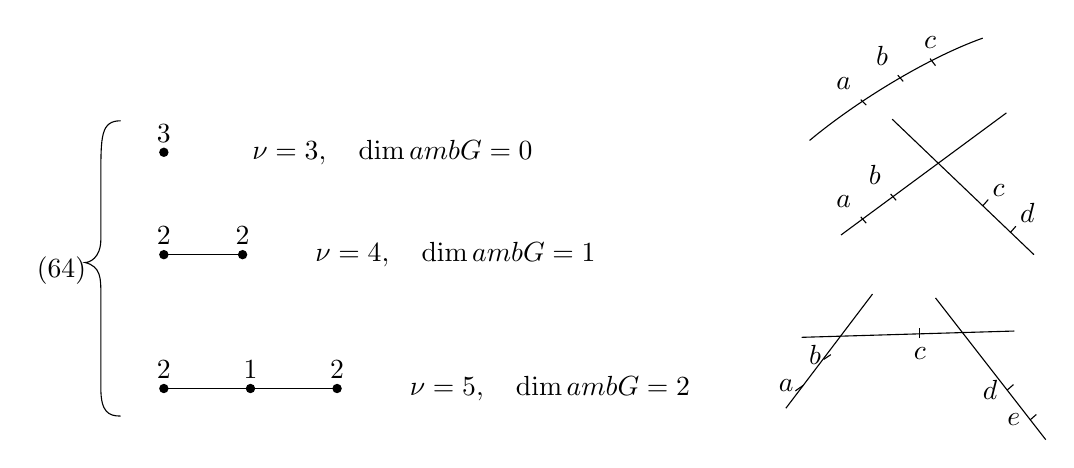
\begin{tikzpicture}[x=1cm,y=1cm]
\node at (-1.3,-1.5) {$(64)$};
\draw (-.55,.4) .. controls (-.8,.4) and (-.8,.2) .. (-.8,-.3) -- (-.8,-1.1) .. controls (-.8,-1.35) and (-.95,-1.4) .. (-1,-1.4) .. controls (-.8,-1.45) and (-.8,-1.6) .. (-.8,-1.8) -- (-.8,-3.0) .. controls (-.8,-3.3) and (-.7,-3.35) .. (-.55,-3.35);
\fill (0,0) circle (1.7pt); \node[above] at (0,0) {$3$};
\node[right] at (1,0) {$\nu=3,\quad\dim\operatorname{amb}G=0$};
\draw (0,-1.3)--(1,-1.3); \fill (0,-1.3) circle (1.7pt); \fill (1,-1.3) circle (1.7pt);\node[above] at (0,-1.3) {$2$};\node[above] at (1,-1.3) {$2$};
\node[right] at (1.8,-1.3) {$\nu=4,\quad\dim\operatorname{amb}G=1$};
\draw (0,-3)--(2.2,-3);\fill (0,-3) circle (1.7pt);\fill (1.1,-3) circle (1.7pt);\fill (2.2,-3) circle (1.7pt);
\node[above] at (0,-3) {$2$};\node[above] at (1.1,-3) {$1$};\node[above] at (2.2,-3) {$2$};\node[right] at (3,-3) {$\nu=5,\quad\dim\operatorname{amb}G=2$};
\draw (8.2,.15) .. controls (8.8,.65) and (9.7,1.2) .. (10.4,1.45);
\draw (8.85,.67)--(8.92,.60);\node[above left] at (8.85,.67) {$a$};\draw (9.32,.98)--(9.39,.90);\node[above left] at (9.32,.98) {$b$};\draw (9.73,1.19)--(9.80,1.10);\node[above] at (9.73,1.19) {$c$};
\draw (8.6,-1.05)--(10.7,.5);\draw (9.25,.42)--(11.05,-1.3);
\draw (8.85,-.82)--(8.92,-.9);\node[above left] at (8.85,-.82) {$a$};\draw (9.23,-.53)--(9.30,-.61);\node[above left] at (9.23,-.53) {$b$};\draw (10.4,-.68)--(10.47,-.60);\node[above right] at (10.4,-.68) {$c$};\draw (10.75,-1.02)--(10.82,-.94);\node[above right] at (10.75,-1.02) {$d$};
\draw (8.1,-2.35)--(10.8,-2.27);\draw (7.9,-3.25)--(9,-1.8);\draw (9.8,-1.85)--(11.2,-3.65);
\draw (8.12,-2.96)--(8.02,-3.03);\node[left] at (8.12,-2.96) {$a$};\draw (8.47,-2.57)--(8.38,-2.63);\node[left] at (8.47,-2.57) {$b$};\draw (9.6,-2.36)--(9.6,-2.23);\node[below] at (9.6,-2.36) {$c$};\draw (10.71,-3.02)--(10.79,-2.95);\node[left] at (10.71,-3.02) {$d$};\draw (11.0,-3.4)--(11.08,-3.33);\node[left] at (11,-3.4) {$e$};
\end{tikzpicture}}
\margin{52}
